\documentclass[pdf]{beamer}
\usepackage{graphicx}
\mode<presentation>{}
\title{LibEuFin}
\subtitle{Libre European Finance}
\author{Marcello Stanisci}

\begin{document}

% Notes:
% What's missing:
% - make clear why this is *civic tech*
%   (e.g.: moving away from 3rd party surveillance,
%    moving away from cloud, taking control of your own (bank transaction) data)
% - make more clear how other civic tech projects can benefit

% Title frame
\begin{frame}
  \titlepage
\end{frame}

\begin{frame}{PSD2, I}
  \begin{center}
  PSD2 is a EU directive about what properties must be fulfilled by
  IT services offered by any financial institution.
  \end{center}
\end{frame}

\begin{frame}{PSD2, II}
  \begin{center}
  it focuses on security and programmatic access to people's assets,
  {\it but} it is concerned about {\it third parties}.
  \end{center}
\end{frame}

\begin{frame}{What does that mean?}
  \begin{center}
  It is all about companies: PSD2 regulates how companies (banks) let
  \underline{other} companies (Fintech provider / Finanzamt / \dots) access
  \textbf{your} assets.
  \end{center}
\end{frame}

\begin{frame}{What can people do?}
  \begin{center}
  Watch.
  \end{center}
\end{frame}

\begin{frame}{Not really..}
  \begin{center}
  Protocols "for people" exist, but are \textbf{a lot}
  and \textbf{difficult}.
  \end{center}
\end{frame}

\begin{frame}{A few examples}
  \begin{itemize}
    \item EBICS: hundreds of pages, just for {\it enclosing} payloads
    \item ISO20022: hundreds of pages for payloads
    \item FinTS / HBCI: hundreds of pages
    \item NextGenPSD2 by Berlin Group 
    \item Startup banks: N26 / Revoult
    \item 100\% proprietary: PayPal
    \item ..
  \end{itemize}
\end{frame}

\begin{frame}{What to do?}
  \begin{center}
  Simplification might lead {\it more people} to use banking APIs,
  resulting in {\it more importance} in decision processes.
  \end{center}
\end{frame}

\begin{frame}{What is LibEuFin}
  \begin{itemize}
  \item {\it Unifies} several banking protocols into an abstraction layer.
  \item Enables development of FinTech apps {\it without clouds or third parties}
  \item {\it Frees} application developers from implementing {\it difficult cryptography}
  \end{itemize}
\end{frame}

\begin{frame}{Architecture}
  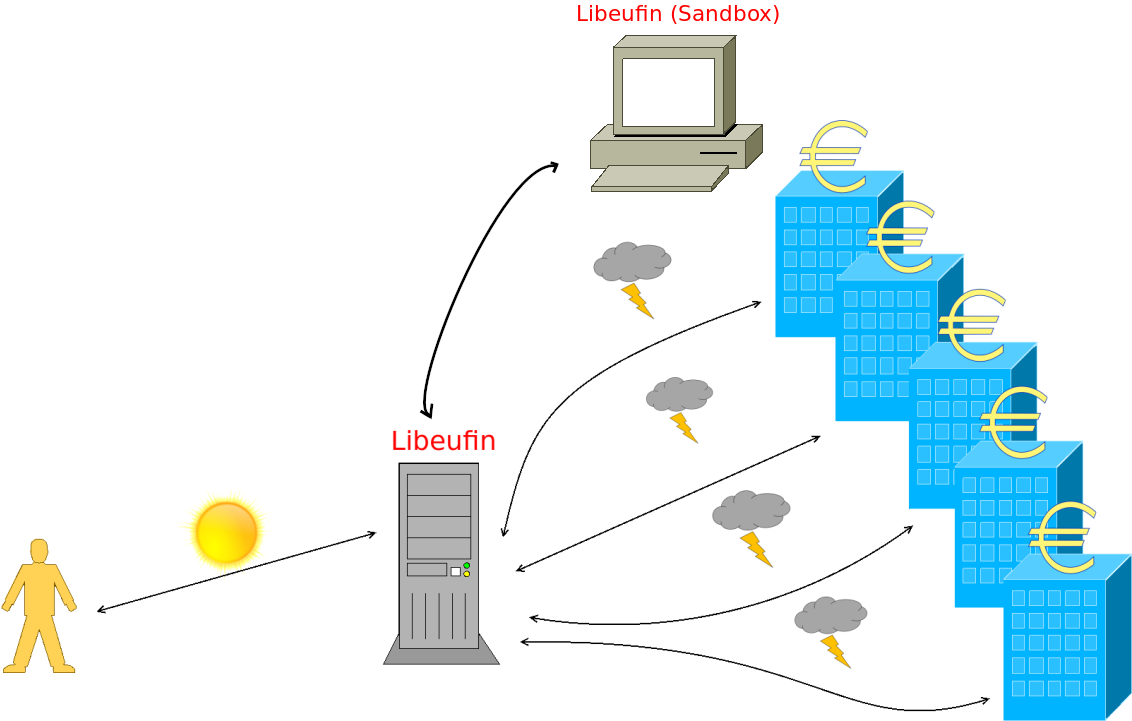
\includegraphics[height=0.63\textheight]{libeufin.png}
\end{frame}

\begin{frame}{What's next?}
  \begin{itemize}
    \item Integration with Taler and GnuCash.
    \item Taler (a former Prototype fund project) found {\it further} funding for the next two years!
  \end{itemize}
\end{frame}

\begin{frame}{Final remark}
  \begin{center}
  We believe that \textbf{simplicity} is the key for any system to
  properly function, and that is LibEuFin primary goal.
  \end{center}
\end{frame}

\end{document}
